\section{Results}

\subsection{Step-by-step Example with OR}
Recall the two bit function OR which returns $1$ if there
is at least a single $1$ in the input and returns $0$ otherwise.
To understand Reichardt's formulation and the conversion
to Boyd's standard form, consider as inputs to our tool
the case with function $f: D \rightarrow E$ where
$D \subseteq {\{0,1\}}^2$ and $E =\{OR(x): x \in D \}$.
Let $F$ be the set of $(y,z)$ such that $f(y) \neq f(z)$. In this
case, $F = \{(00,01), (00,10), (00,11), (01,00), (10,00), (11,00)\}$

Let
\begin{align}
\X = \begin{blockarray}{ccccc}
\qquad & 00 & 01 & 10 & 11 \\
\begin{block}{c[cccc]}
  00 & X_{(00,00)} & X_{(00,01)} & X_{(00,10)} & X_{(00,11)}\\
  01 & X_{(01,00)} & X_{(01,01)} & X_{(01,10)} & X_{(01,11)}\\
  10 & X_{(10,00)} & X_{(10,01)} & X_{(10,10)} & X_{(10,11)}\\
  11 & X_{(11,00)} & X_{(11,01)} & X_{(11,10)} & X_{(11,11)}\\
\end{block}
\end{blockarray}. \nonumber 
\end{align}


The objective function of the SDP is
\begin{align} \label{eq:reichardtObj} 
    f_{\text{bound}} &= M(\X) = \max_{y \in D} \sum_{j \in [n]}
    \bra{y,j}\X\ket{y,j} \nonumber \\
    &= \max\{ \tr{X_{(00,00)}}, \tr{X_{(01,01)}}, \tr{X_{(10,10)}}, \tr{X_{(11,11)}} \} \nonumber
\end{align}
subject to constraints
\begin{align}
    \X \succcurlyeq 0  \nonumber 
\end{align}
and
\begin{align}\label{specific_constraint}
    \forall (y,z) \in F \sum_{j \in [n]: y_j \ne z_j} 
    \bra{y,j} \X \ket{z, j} = 1.
\end{align}
Observe that \cref{specific_constraint}
is equivalent to
\begin{align}
    \tr{X_{(00,01)}} &= \tr{X_{(00,10)}} = \tr{X_{(00,11)}} = 1 \nonumber \\
    \tr{X_{(01,00)}} &= \tr{X_{(10,00)}} = \tr{X_{(11,00)}} = 1. \nonumber
\end{align}

Our goal is to minimize $M$, 
and thus $f_{\text{bound}}$ by 
finding the optimal value of $\X$. 
By running our SDP solver, we obtain 
$\X$ with an objective function value of $\sqrt{2}$.
\begin{align}
    \X = \left[ \begin{array}{cc|cc|cc|cc}
    0.7 & 0 & 0 & 0 & 1 & 0 & 0.5 & 0\\
    0 & 0.7 & 0 & 1 & 0 & 0 & 0 & 0.5\\
    \hline
    0 & 0 & 0 & 0 & 0 & 0 & 0 & 0\\
    0 & 1 & 0 & \sqrt{2} & 0 & 0 & 0 & 0.7\\
    \hline
    1 & 0 & 0 & 0 & \sqrt{2} & 0 & 0.7 & 0\\
    0 & 0 & 0 & 0 & 0 & 0 & 0 & 0\\
    \hline
    0.5 & 0 & 0 & 0 & 0.7 & 0 & 0.6 & 0\\
    0 & 0.5 & 0 & 0.7 & 0 & 0 & 0 & 0.6\\
    \end{array}
\right] \nonumber
\end{align}
We use our solution to construct the input
vectors to the span program.
Consider $L$ such that $L^\dagger L = \X$.
Then construct $\bra{v_{x,i}}$
for all $x \in D$, $i \in [n]$.
With \cref{input_vectors},
\begin{align}
I &= \left[\begin{array}{cc}
    \bra{1}\bra{v_{00,1}} & \bra{1}\bra{v_{00,2}} \\
    \bra{1}\bra{v_{01,1}} & \bra{0}\bra{v_{01,2}} \\
    \bra{0}\bra{v_{10,1}} & \bra{1}\bra{v_{10,2}}\\
    \bra{0}\bra{v_{11,1}} & \bra{0}\bra{v_{11,2}}\\
\end{array} \right] \nonumber \\
&= \left[\begin{array}{c|c|c|c}
    0 \cdots 0 & \bra{v_{00,1}} & 0 \cdots 0 & \bra{v_{00,2}} \\
    0 \cdots 0 & \bra{v_{01,1}} & \bra{v_{01,2}} & 0 \cdots 0\\
    \bra{v_{10,1}} & 0 \cdots 0 & 0 \cdots 0 & \bra{v_{10,2}}\\
    \bra{v_{11,1}} & 0 \cdots 0 & \bra{v_{11,2}} & 0 \cdots 0\\
\end{array} \right] \nonumber
\end{align}
The columns of $I$ are the columns
used in the span program. 
If we remove rows of $I$ corresponding to elements 
$ x \in D$ such that $f(x) = 1$
and columns of $I$ that are the 
all zero vector, we obtain an equivalent span program where
\begin{align}
I &= \left[\begin{array}{cccc}
   0 & 1 & 0 & 1 \\
\end{array} \right] \nonumber
\end{align}
and $\tau = 1$.
In both definitions of $I$, the left two partitions
correspond to the first bit in the
input, and the right two partitions correspond 
to the second bit of the input. For each
input bit, the relevant block of $I$ 
is broken into left and right halves, corresponding
to whether the bit is $0$ (left) or $1$ (right). 
It is clear from this matrix that if either input bit is
$1$ the function will return true and otherwise
will return false.

\subsection{Accuracy with OR and Parity}

\begin{figure}[H]
\centering
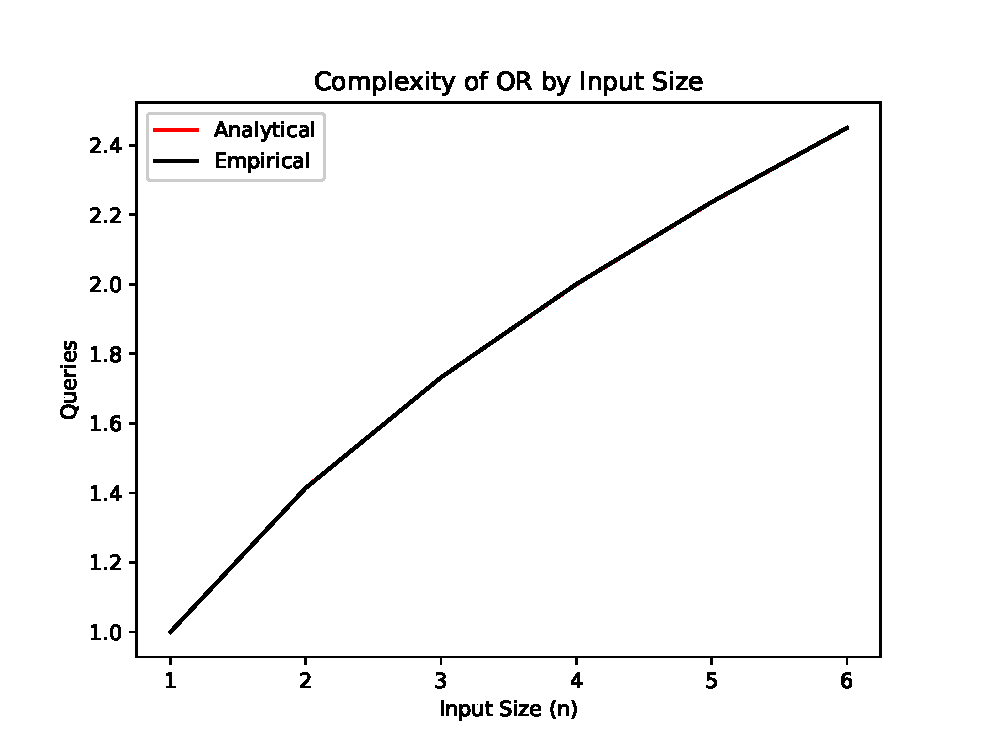
\includegraphics[scale=.5]{or_complexity}
\caption{The proven analytical optimal query complexity
and calculated empirical optimal query complexity by 
size of input bitstring for OR.}
\label{fig:or_complexity}
\end{figure}

We verify that the implementation works correctly
with results for OR on various input sizes.
The optimal quantum query complexity of OR
is $\sqrt{n}$ and, as demonstrated in
\cref{fig:or_complexity},
we the empirical results match the analytical
to the thousandth place.

\begin{figure}[H]
\centering
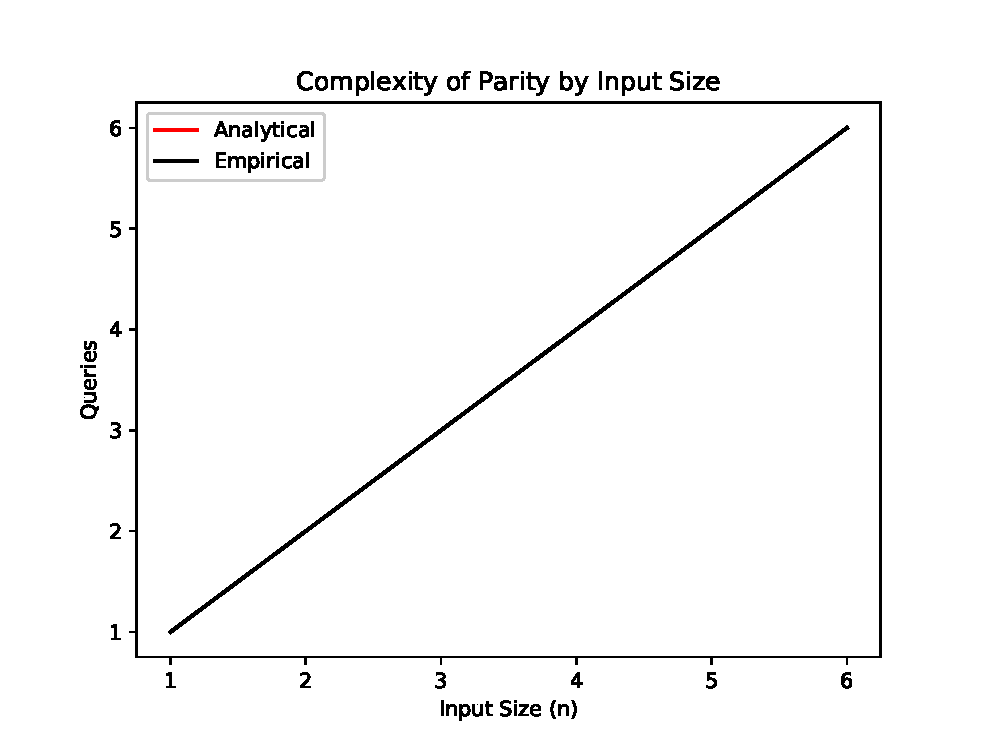
\includegraphics[scale=.5]{parity_complexity}
\caption{The proven analytical optimal query complexity
and calculated empirical optimal query complexity by 
size of input bitstring for parity.}
\label{fig:parity_complexity}
\end{figure}

The parity function, determining whether
there are an even number of 1's an input
bitstring, is known to have optimal
quantum query complexity linear to the number of bits.
The implementation also correctly
calculates the complexity of parity to the thousandth
place as demonstrated in \cref{fig:parity_complexity}.

The results for OR and parity demonstrate
that the implementation accurately calculates
optimal quantum query complexity.

\subsection{Runtime with OR}

\begin{figure}[H]
\centering
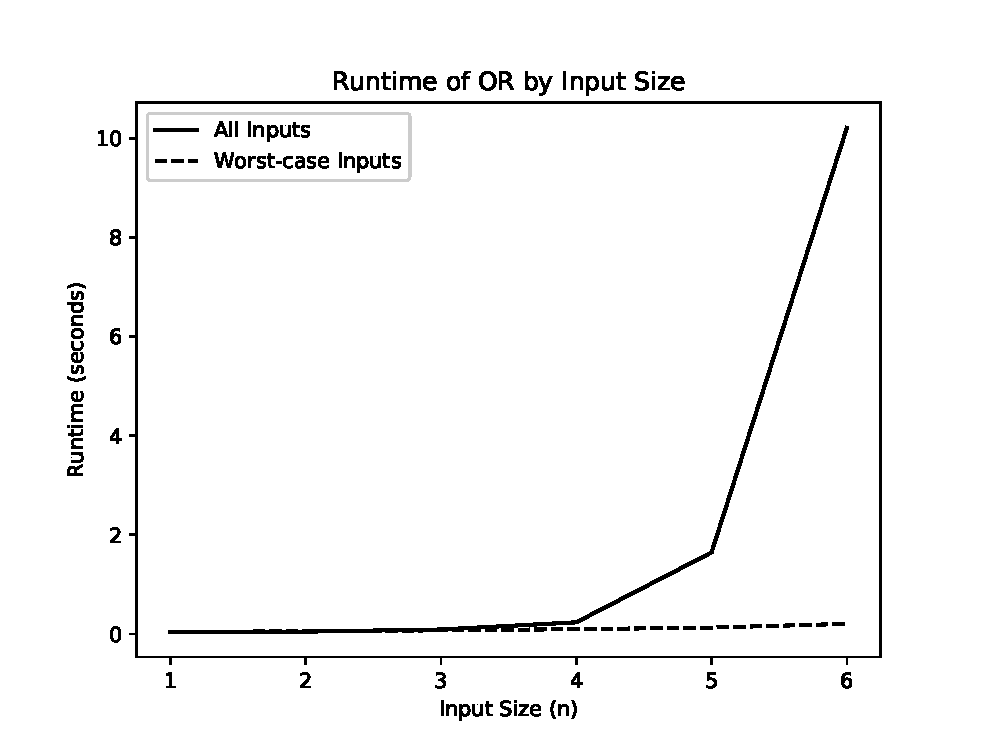
\includegraphics[scale=.5]{or_runtime}
\caption{Runtime of SDP solver by size of input strings.}
\label{fig:or_runtime}
\end{figure}

Recall that the size of the input to the implementation
does not have to be all $2^n$ input bitstrings
for input size $n$. In fact,
by choosing different and smaller inputs,
we can improve runtime while maintaining accuracy.

In \cref{fig:or_runtime}, observe that the
runtime of the implementation on OR with all
inputs increases exponentially
with the input size $n$.
(Since the number of inputs grows exponentially,
it follows that the size of the problem grows
exponentially, too.)
The bottleneck in the implementation is
the eigenvalue decomposition of the current
solution at each step of the iteration.
However, if we limit the inputs to the `worst-case`
bitstrings we observe much lower runtimes.
It is in general very difficult to find the worst-case
inputs and OR is a special case.
When searching for at least one 1, the most
difficult bitstrings to search are those with a single 1.
So, by supplying only the worst-case inputs that
have at most one 1, we can maintain accuracy while
greatly reducing runtime.
We know of no other Boolean functions with
similarly intuitive worst-case sets of inputs.
